\documentclass[../main.tex]{subfiles}
\begin{document}
\section{定位问题}
\subsection{定位问题的基本概念}
\begin{enumerate}
    \item \textbf{定位}:确定机器人在\textbf{世界}(全局)坐标系中的位置/位姿
\end{enumerate}
\subsection{基于外部设备感知的定位}
\begin{enumerate}
    \item \textbf{全球定位系统GPS}
    \begin{itemize}
        \item \textbf{GPS(Global Positioning System)}:由\textbf{空间端}\footnote{24颗卫星位于6个倾角为55度的轨道平面内,每个轨道平面内4颗卫星,高度20182千米,周期12小时}、\textbf{控制端}\footnote{包括1个主控站、1个备用主控站、4个地面天线站和6个监测站,主要作用监测控制卫星的运行,并对卫星进行时间同步}和\textbf{用户端}\footnote{卫星接收到信号,根据信号发射时间和接收时间差计算接收器和卫星之间的距离}三部分组成,也称为GNSS (Global Navigation Satellite System)
            \begin{figure}[H]
                \centering
                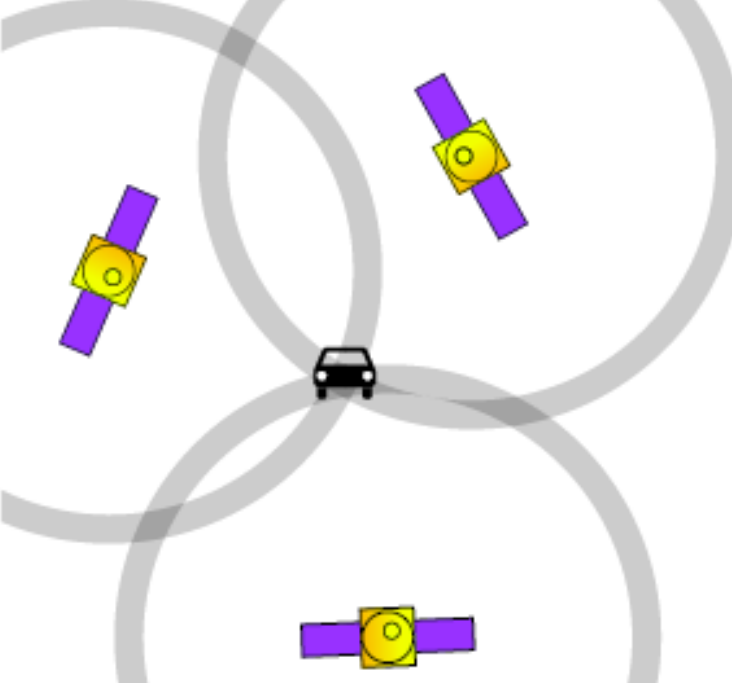
\includegraphics[width=0.3\textwidth]{images/gps.png}
                \caption{三点定位法}
            \end{figure}
        {\small\kaishu Q:为什么至少需要四个卫星的信号实现最优估计?\\A:电磁波传播速度等同于光束,因此,
时钟精度会极大地影响定位精度:
    \begin{itemize}
        \item 卫星时钟采用原子钟,精度高
        \item 接收器时钟采用石英钟,通常不够精确
    \end{itemize}
在估计用户端位置时,有必要同时估计接收器时钟误差,即估计状态为\( \mathbf{x} = {\left( x,y,z,{\delta }_{\text{clock }}\right) }^{T} \)}
        \item \textbf{差分全球定位系统 DGPS (DIFFERENTIAL GPS)}:消除GPS系统中出于利益考虑被人为引入的误差,基本原理是:
            \begin{itemize}
                \item 在位置精确测定的已知点上配备一台GPS接收机作为基准站
                \item 基准站将GPS观测结果与基准站坐标比较,求解出\textbf{实时差分修正值},广播给附近用户
            \end{itemize}
        \item \textbf{缺点}:
        \begin{itemize}
            \item 遮挡问题,室内难以使用
            \item 多路径问题
        \end{itemize}
        \begin{figure}[H]
    \centering
        \begin{subfigure}[b]{0.35\textwidth}
            \centering
            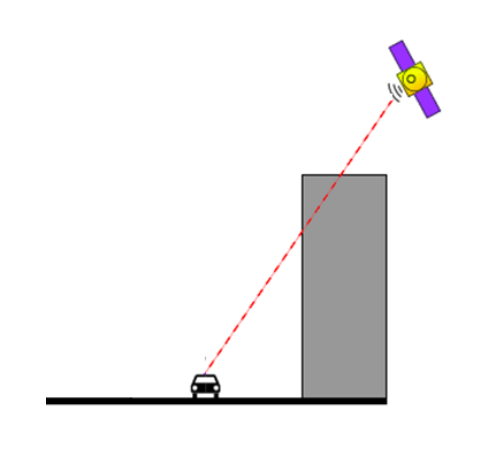
\includegraphics[width=\textwidth]{images/hide.png}
            \caption{遮挡问题}
            \label{fig:hide}
        \end{subfigure}
        \begin{subfigure}[b]{0.48\textwidth}
            \centering
            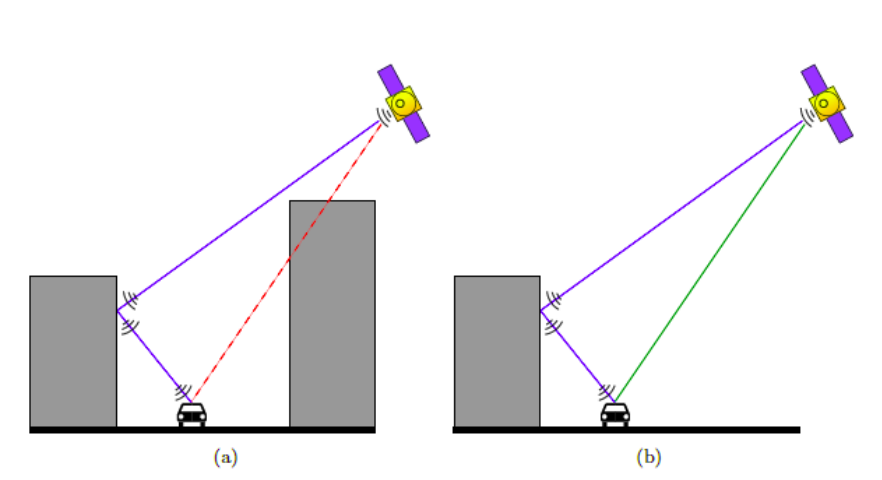
\includegraphics[width=\textwidth]{images/multipath.png}
            \caption{多路径问题}
            \label{fig:multipath}
        \end{subfigure}
        \caption{全球定位系统的问题}
        \label{fig:gps_issues}
    \end{figure}
    \end{itemize}
    \item \textbf{全局视觉观测定位}
            \begin{figure}[H]
                \centering
                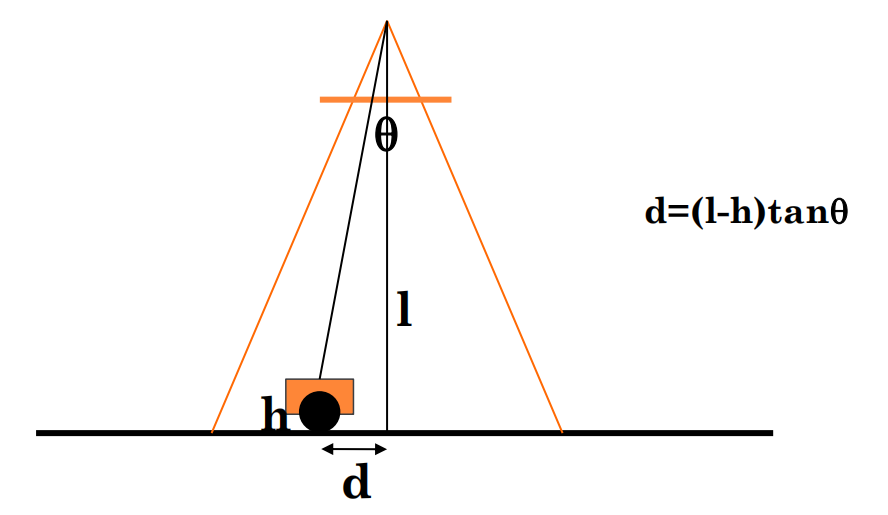
\includegraphics[width=0.5\textwidth]{images/visonlocate.png}
                \caption{视觉定位,如果需要更大的视野,则架设多个相机}
            \end{figure}
    \begin{itemize}
        \item \textbf{基本思想}:搭建一套外部视觉系统,识别机器人,确定其位置
        \item \textbf{应用约束}:
        \begin{itemize}
            \item 摄像头有\textbf{视野范围约束},当环境较大时需要多个摄像头
            \item 机器人上需要有一定的\textbf{标识}方便图像识别定位
        \end{itemize}
    \end{itemize}
    \item \textbf{成本分析}
    \begin{itemize}
        \item 机器人本体实现简单,直接接受定位结果,可降低成本
        \item 外部感知系统成本较高,且感知范围越大,成本越高
    \end{itemize}
\end{enumerate}
\subsection{基于本体感知的定位}
\begin{enumerate}
            \begin{figure}[H]
                \centering
                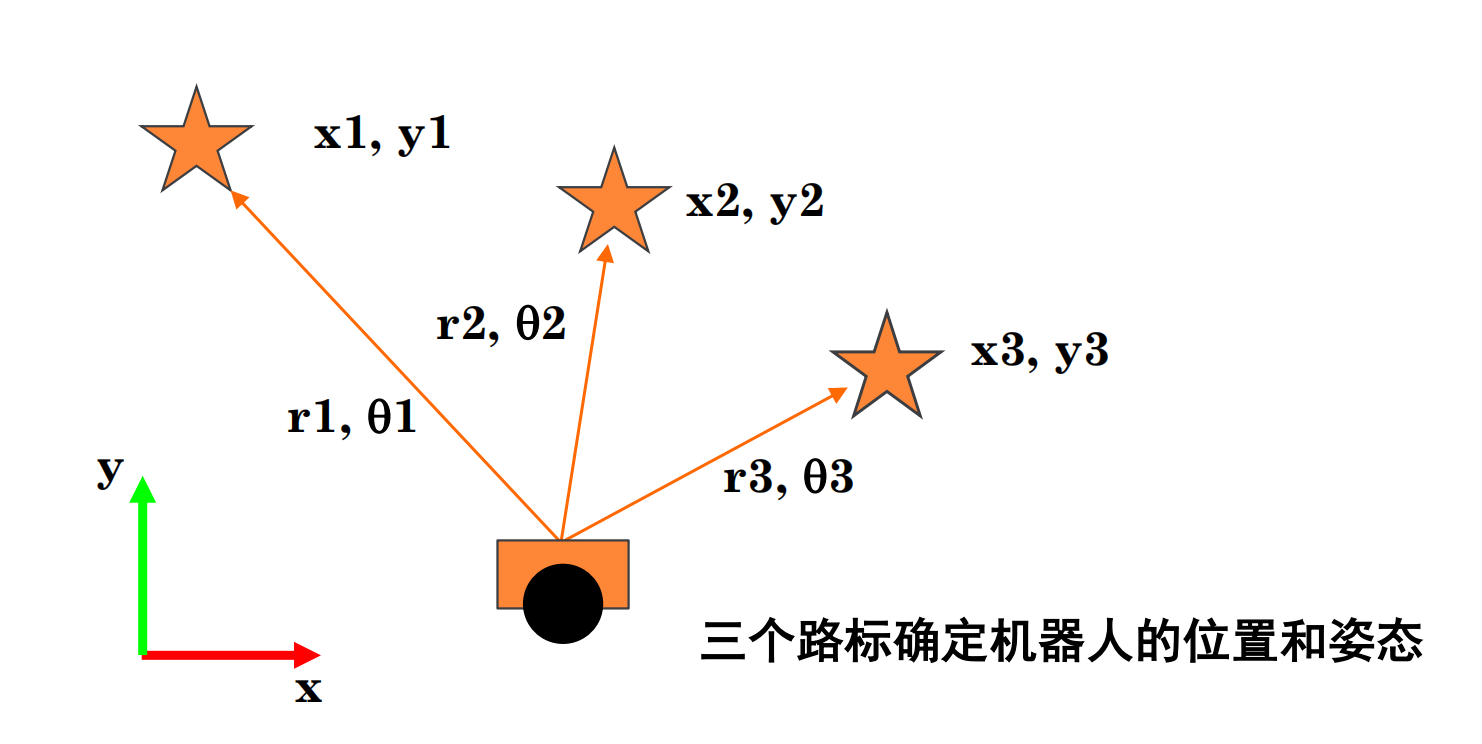
\includegraphics[width=0.5\textwidth]{images/3lubiao.png}
                \caption{三个路标确定机器人的位置和姿态}
            \end{figure}
    \item \textbf{基于空间标识的定位}
        \begin{itemize}
            \item \textbf{基于环境人工标识的定位}:在环境中部署特殊标签,降低成本,确保可靠性
                \begin{itemize}
                    \item 地面二维码
                    \item 激光反射板
                \end{itemize}
            \item \textbf{基于环境自然标识的定位}
        \end{itemize}
    \item \textbf{基于位置识别的定位}
        \begin{itemize}
            \item \textbf{基本思想}:利用本体传感器获得的信息与地图中存储的各个位置上的信息进行匹配,实现位置识别
            \item \textbf{应用约束}:
            \begin{itemize}
                \item 环境的\textbf{动态变化}和不同位置的\textbf{相似性},对位置辨别带来挑
                \item 战为适应环境的动态变化,可以考虑对每个位置存储\textbf{多张图片},但增加存储空间需求
                \item 图像匹配是一个\textbf{耗时}的工作
            \end{itemize}
        \end{itemize}
    \item \textbf{特点}
    \begin{itemize}
        \item 需要\textbf{预先构建地图},地图坐标系在构建地图时确定
        \item 对于大规模环境,路标需具备\textbf{可鉴别性},否则需要正确的数据关联
        \item 存储大规模环境的图片需要较大的\textbf{存储空间}
        \item 对于实际环境中存在路标被破坏/污染、更换、稀疏等风险
    \end{itemize}
        
\subsection{控制感知信息融合的的自定位}
\begin{enumerate}
    \item \textbf{基本概念}:给定环境地图(对环境的已有知识)的条件下,根据机器人的运动控制/里程估计信息和传感器感知数据(当前认知)估计机器人相对于环境地图的坐标。
    \item \textbf{问题分类}:
    \begin{enumerate}
        \item \textbf{位置跟踪(position tracking)}:机器人初始位置已知,需要解决对里程计累积误差的补偿
        \item \textbf{全局定位(global localization)}:机器人初始位置未知
        \item \textbf{绑架问题(kidnapped robot problem)}:机器人在定位良好的条件下突然被移到另一个未被告知的地方\footnote{与全局定位问题的差异在于,当机器人被绑架时,机器人可能已经对自已所在的位置非常确信了},用于检测定位算法发现错误并从错误中恢复的能
    \end{enumerate}
    \item \textbf{简单方法}:根据观测进行定位,没有观测根据里程估计进行航位推算
        \begin{itemize}
            \item \textbf{缺点}:如何融合?
                \begin{itemize}
                    \item 观测存在不确定性,里程估计也存在不确定性,如何\textbf{融合是否观测}
                    \item 观测到多个特征(例如多个交通标志)时,如何\textbf{融合多个观测}进行估
                \end{itemize}
            \item \textbf{解决方案}:
                \begin{itemize}
                    \item 对不确定性进行描述(称为\textbf{置信度}),在\textbf{概率架构}下进行融合
                    \item 用\textbf{方差}表示置信度,方差小表示置信度高
                    \item 控制感知信息融合的自定位就是利用里程估计和观测信息估计\textbf{方差最小}下的机器人位姿
                \end{itemize}
        \end{itemize}
    \item \textbf{概率描述}:定位问题可以定义为\textbf{最优估计问题},最优估计的一个体现是估计的方差很小——用贝叶斯估计器\textbf{是一种最小方差估计器}\\
            我们希望计算:
        \[
        \widehat{\mathbf{X}}^{t} \triangleq \mathbb{E}\left[ \mathbf{X}^{t} \mid \mathbf{Z}^{t}, \mathbf{U}^{t-1}, \mathbf{m} \right]
        \]
        即在给定当前时刻以及历史所有观测$\mathbf{Z}^{t}$、上一时刻以及之前所有控制$\mathbf{U}^{t-1}$,以及地图$\mathbf{m}$后,路径的$\mathrm{x}^t$最优估计。
        {\small\kaishu 
        \begin{enumerate}
        \item \textbf{问题定义}:\\
        记地图为 \( \mathrm{m} \) ,\\
\( t \) 时刻机器人位姿为 \( \mathrm{x}_{t} = {\left( {x}_{t},{y}_{t},{\theta }_{t}\right) }^{T} \) ,\\观测信息为 \( {z}_{t} \) ,\\控制信息为 \( {u}_{t} \)\\路径、观测和控制的历史集合定义:
\( {\mathbf{X}}^{t} = \left\{  {{\mathbf{x}}_{0},{\mathbf{x}}_{1},\ldots ,{\mathbf{x}}_{t}}\right\}  \;{\mathbf{Z}}^{t} = \left\{  {{\mathbf{z}}_{0},{\mathbf{z}}_{1},\ldots ,{\mathbf{z}}_{t}}\right\}  \;{\mathbf{U}}^{t - 1} = \left\{  {{\mathbf{u}}_{0},{\mathbf{u}}_{1},\ldots ,{\mathbf{u}}_{t - 1}}\right\} \)
\\求 \( {\widehat{\mathbf{X}}}^{t} \triangleq  \mathbf{E}\left\lbrack  {{\mathbf{X}}^{t} \mid  {\mathbf{Z}}^{t},{\mathbf{U}}^{t - 1},\mathbf{m}}\right\rbrack \)
        \item \textbf{递推关系推导:}\footnote{我们希望在每个时刻只用上一步的结果来更新,通过该递推关系,我们可以实现概率意义下的自定位}
        
        从联合概率出发,根据乘法公式:
        \[
        p(X,Y) = p(Y \mid X) p(X)
        \]
        可得:
        \[
        p(\mathbf{X}^{t} \mid \mathbf{Z}^{t}, \mathbf{U}^{t-1}, \mathbf{m})
        = p(\mathbf{x}_t \mid \mathbf{X}^{t-1}, \mathbf{Z}^{t}, \mathbf{U}^{t-1}, \mathbf{m})
        \, p(\mathbf{X}^{t-1} \mid \mathbf{Z}^{t}, \mathbf{U}^{t-1}, \mathbf{m})
        \]
        
        因为 \( \mathbf{X}^{t-1} \) 与之后的观测、控制无关:
        \[
        p(\mathbf{X}^{t-1} \mid \mathbf{Z}^{t}, \mathbf{U}^{t-1}, \mathbf{m})
        = p(\mathbf{X}^{t-1} \mid \mathbf{Z}^{t-1}, \mathbf{U}^{t-2}, \mathbf{m})
        \]
        故:
        \[
        p(\mathbf{X}^{t} \mid \mathbf{Z}^{t}, \mathbf{U}^{t-1}, \mathbf{m})
        = p(\mathbf{x}_t \mid \mathbf{X}^{t-1}, \mathbf{Z}^{t}, \mathbf{U}^{t-1}, \mathbf{m})
        \, p(\mathbf{X}^{t-1} \mid \mathbf{Z}^{t-1}, \mathbf{U}^{t-2}, \mathbf{m})
        \]
        
        \item \textbf{引入贝叶斯公式:}
        \[
        p(Y \mid X) = \eta \, p(X \mid Y)p(Y)
        \]
        (其中 \(\eta\) 为归一化常数。)
        
        得:
        \[
        p(\mathbf{X}^{t} \mid \mathbf{Z}^{t}, \mathbf{U}^{t-1}, \mathbf{m})
        = \eta \, p(\mathbf{z}_t \mid \mathbf{X}^{t}, \mathbf{Z}^{t-1}, \mathbf{U}^{t-1}, \mathbf{m})
        \, p(\mathbf{x}_t \mid \mathbf{X}^{t-1}, \mathbf{Z}^{t-1}, \mathbf{U}^{t-1}, \mathbf{m})
        \, p(\mathbf{X}^{t-1} \mid \mathbf{Z}^{t-1}, \mathbf{U}^{t-2}, \mathbf{m})
        \]
        
        \item \textbf{根据马尔可夫假设(系统独立性)简化:}
        \begin{enumerate}
            \item 当前状态仅依赖于上一时刻状态与控制量:
            \[
            p(\mathbf{x}_t \mid \mathbf{X}^{t-1}, \mathbf{Z}^{t-1}, \mathbf{U}^{t-1}, \mathbf{m})
            = p(\mathbf{x}_t \mid \mathbf{x}_{t-1}, \mathbf{u}_{t-1}, \mathbf{m})
            \]
            \item 当前观测仅依赖于当前状态:
            \[
            p(\mathbf{z}_t \mid \mathbf{X}^{t}, \mathbf{Z}^{t-1}, \mathbf{U}^{t-1}, \mathbf{m})
            = p(\mathbf{z}_t \mid \mathbf{x}_t, \mathbf{m})
            \]
        \end{enumerate}
        
        将上述代入后,得到最终递推形式:
        \[
        \boxed{
        p(\mathbf{X}^{t} \mid \mathbf{Z}^{t}, \mathbf{U}^{t-1}, \mathbf{m})
        = \eta \, p(\mathbf{z}_t \mid \mathbf{x}_t, \mathbf{m})
        \, p(\mathbf{x}_t \mid \mathbf{x}_{t-1}, \mathbf{u}_{t-1}, \mathbf{m})
        \, p(\mathbf{X}^{t-1} \mid \mathbf{Z}^{t-1}, \mathbf{U}^{t-2}, \mathbf{m})
        }
        \]
        分别代表:\\
        - \( p(\mathbf{X}^{t} \mid \mathbf{Z}^{t}, \mathbf{U}^{t-1}, \mathbf{m}) \):t时刻的后验分布\\
        - \( p(\mathbf{z}_t \mid \mathbf{x}_t, \mathbf{m}) \):观测模型\\
        - \( p(\mathbf{x}_t \mid \mathbf{x}_{t-1}, \mathbf{u}_{t-1}, \mathbf{m}) \):运动模型  \\
        - \( p(\mathbf{X}^{t-1} \mid \mathbf{Z}^{t-1}, \mathbf{U}^{t-2}, \mathbf{m}) \):t-1时刻的后验分布
        
        
        \item \textbf{状态量化形式:}
        实际应用中,我们通常只关心当前位姿的后验,而非整条路径:
        \[
        \mathbf{x}_t = \mathbb{E}\left[\mathbf{x}_t \mid \mathbf{Z}^{t}, \mathbf{U}^{t-1}, \mathbf{m}\right]
        \]
        对应概率递推形式为:
        \[
        p(\mathbf{x}_t \mid \mathbf{Z}^{t}, \mathbf{U}^{t-1}, \mathbf{m})
        = \eta \, p(\mathbf{z}_t \mid \mathbf{x}_t, \mathbf{m})
        \int p(\mathbf{x}_t \mid \mathbf{x}_{t-1}, \mathbf{u}_{t-1}, \mathbf{m})
        \, p(\mathbf{x}_{t-1} \mid \mathbf{Z}^{t-1}, \mathbf{U}^{t-2}, \mathbf{m})
        \, d\mathbf{x}_{t-1}
        \]
        该公式被称为\textbf{实时自定位贝叶斯递推公式}。
        
        \end{enumerate}
        }
    \end{enumerate}
\end{enumerate}
\subsection{马尔可夫定位中的运动模型}
        在上一节,我们得到了实时自定位贝叶斯递推公式
        \[
        p(\mathbf{x}_t \mid \mathbf{Z}^{t}, \mathbf{U}^{t-1}, \mathbf{m})
        = \eta \, p(\mathbf{z}_t \mid \mathbf{x}_t, \mathbf{m})
        \int \textcolor{red}{p(\mathbf{x}_t \mid \mathbf{x}_{t-1}, \mathbf{u}_{t-1}, \mathbf{m})}
        \, p(\mathbf{x}_{t-1} \mid \mathbf{Z}^{t-1}, \mathbf{U}^{t-2}, \mathbf{m})
        \, d\mathbf{x}_{t-1}
        \]
        对红色项,利用贝叶斯规则
        $$\textcolor{red}{p(\mathbf{x}_t \mid \mathbf{x}_{t-1}, \mathbf{u}_{t-1}, \mathbf{m})}=\eta     \textcolor{blue}{p(\mathrm{m}|\mathrm{x}_t,\mathrm{x}_{t-1},\mathrm{u}_{t-1})}\textcolor{orange}{p(\mathrm{x}_t|\mathrm{x}_{t-1},\mathrm{u}_{t-1})}$$
        \begin{itemize}
            \item 橙色项:给定上一时刻位姿$x_{t-1}$和控制指令$u_{t-1}$,计算当前位姿$x_{t}$的概率分布,称之为\textbf{概率运动模型}
            \item 蓝色项:在控制指令$u_{t-1}$下机器人从$x_{t-1}$移动到$x_{t}$,在这样条件下地图$m$的可能性\footnote{如果路径或者$x_t$与环境障碍物碰撞,则获得地图$m$的可能性低。通过路径验证地图存在的可能性,实现地图条件下当前位姿估计的验证}
            \begin{figure}[H]
                \centering
                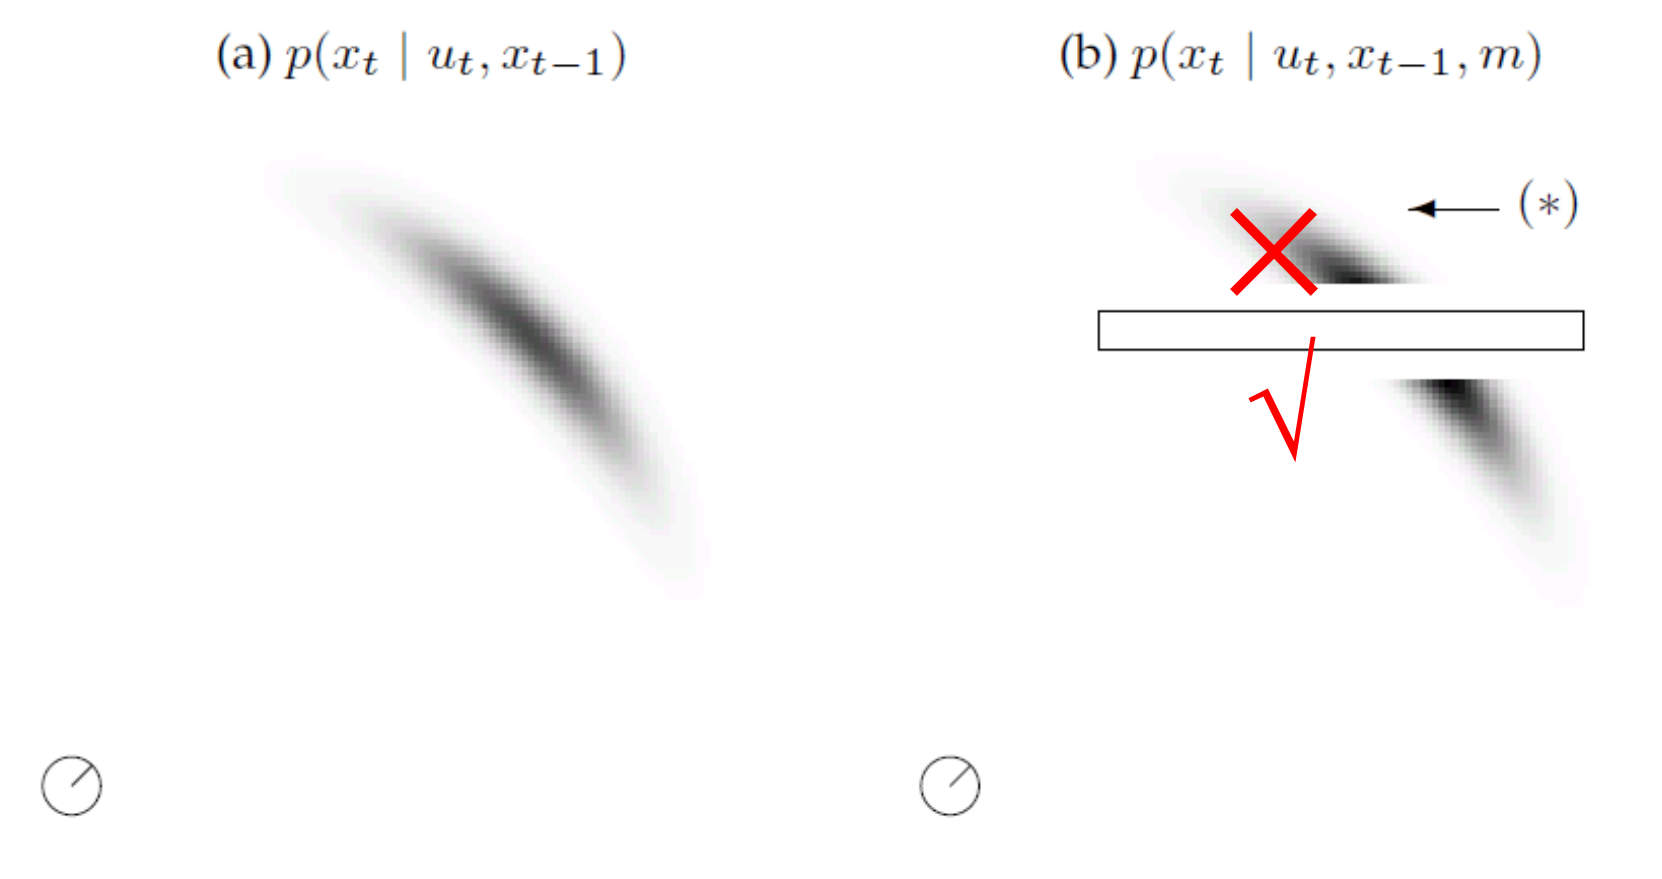
\includegraphics[width=0.3\textwidth]{images/map.png}
                \caption{考虑地图的运动模型}
            \end{figure}
            {\small\kaishu 
            $$ \mathbf{p}\left( {{\mathrm{x}}_{t} \mid  {\mathrm{x}}_{t - 1},{\mathbf{u}}_{t - 1},\mathbf{m}}\right)  = \mathbf{m}\left( {\mathbf{m} \mid  {\mathrm{x}}_{t},{\mathrm{x}}_{t - 1},{\mathbf{u}}_{t - 1}}\right) \mathbf{p}\left( {{\mathrm{x}}_{t} \mid  {\mathrm{x}}_{t - 1},{\mathbf{u}}_{t - 1}}\right)$$
            地图分为可通行和不可通行\\
            本项作用: 基于地图降低运动模型的不确定性\\
            问题:需要融合两次位姿之间路径不被占用的可能性和机器人根据控制跟随该路径的可能性,计算非常复杂,难以计算闭式解\\
            实际应用时,可以
            $$ p\left( {{\mathbf{x}}_{t} \mid  {\mathbf{x}}_{t - 1},{\mathbf{u}}_{t - 1},\mathbf{m}}\right)  \approx  p\left( {{\mathbf{x}}_{t} \mid  {\mathbf{x}}_{t - 1},{\mathbf{u}}_{t - 1}}\right) $$
            $$ p\left( {{\mathbf{x}}_{t} \mid  {\mathbf{x}}_{t - 1},{\mathbf{u}}_{t - 1},\mathbf{m}}\right)  \approx  {\eta p}\left( {{\mathbf{x}}_{t} \mid  {\mathbf{x}}_{t - 1},{\mathbf{u}}_{t - 1}}\right) p\left( {{\mathbf{x}}_{t} \mid  \mathbf{m}}\right) $$
            }
        \end{itemize}
        显然,当采用不同的控制指令即不同的$u$时,概率运动模型也是不同的。接下来,我们分别从
        \begin{itemize}
            \item \textbf{里程计运动模型}:$u_{t-1}$是\textbf{里程估计数据},回顾其航位推算计算公式:
            $$\begin{cases}x_t=x_{t-1}+\Delta d\cos(\theta_{t-1}+\Delta\theta)\\y_t=y_{t-1}+\Delta d\sin(\theta_{t-1}+\Delta\theta)\\\theta_t=\theta_{t-1}+\Delta\theta\end{cases}$$
            \item \textbf{速度运动模型}:$u_{t-1}$是\textbf{控制机器人运动的指令},回顾其航位推算计算公式:
            $$\left.\left(\begin{array}{c}x'\\y'\\\theta'\end{array}\right.\right)=\left(\begin{array}{c}x-\frac{\nu}{\omega}\sin(\theta)+\frac{\nu}{\omega}\sin(\theta+\omega\Delta t)\\y+\frac{\nu}{\omega}\cos(\theta)-\frac{\nu}{\omega}\cos(\theta+\omega\Delta t)\\\theta+\omega\Delta t\end{array}\right)$$
        \end{itemize}
\begin{enumerate}
    \item \textbf{里程计运动模型}\\
    我们的最终目的是计算出$$p(\mathrm{x}_t|\mathrm{x}_{t-1},\mathrm{u}_{t-1})$$
    在里程计运动模型中,我们认为$\mathrm{u}_{t-1}$是$\boldsymbol{\delta} = (\delta_{rot1}, \delta_{trans}, \delta_{rot2})^T$
                \begin{figure}[H]
                \centering
                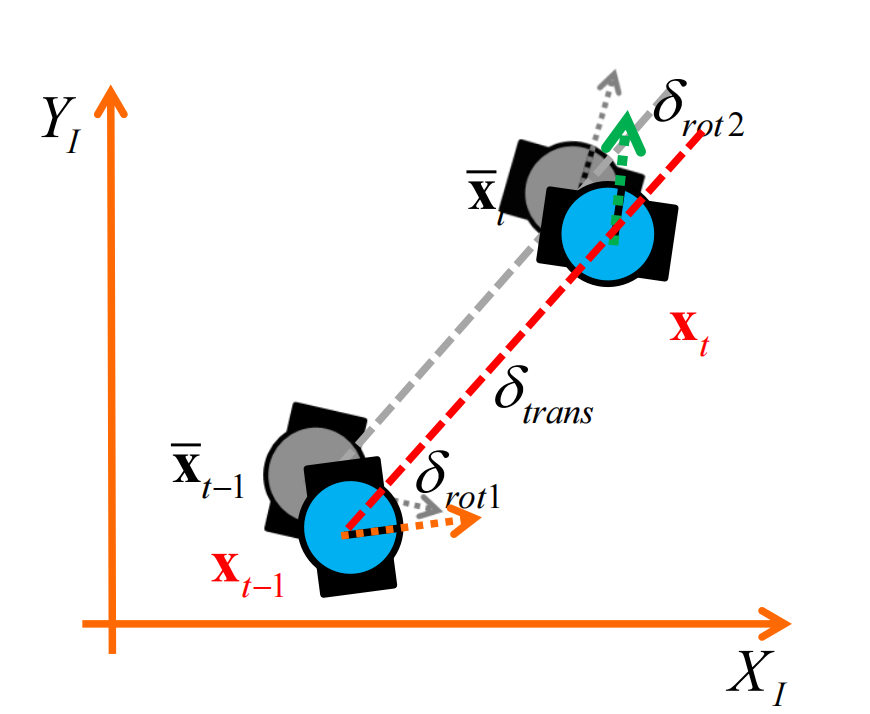
\includegraphics[width=0.3\textwidth]{images/licheng_model1.png}
                \caption{里程计运动模型变量假设}
            \end{figure}
    \begin{enumerate}
        \item \textbf{理想(无噪声)状态下的航位变化}\\
        我们假设机器人先旋转$\delta_{rot1}$、平移$\delta_{trans}$、再旋转$\delta_{rot2}$,将运动变化量        
        
        $$\boldsymbol{\delta} = (\delta_{rot1}, \delta_{trans}, \delta_{rot2})^T$$
        
        叠加到$\mathbf{x}_{t-1}=(x,y,\theta)^T\text{得到}\mathbf{x}_t=(x',y',\theta')^T$
        $$\begin{pmatrix}x'\\y'\\\theta'\end{pmatrix}=\begin{pmatrix}x+\delta_{trans}\cos(\theta+\delta_{rot1})\\y+\delta_{trans}\sin(\theta+\delta_{rot1})\\\theta+\delta_{rot1}+\delta_{rot2}\end{pmatrix}$$

        \item \textbf{不理想(有噪声)状态下的航位变化}\\
        显然,实际测量中是带有各种原因导致的误差的,这里的$$\boldsymbol{\delta} = (\delta_{rot1}, \delta_{trans}, \delta_{rot2})^T$$
        考虑误差后,用头尖尖表示真实值,用波浪线代表误差,不戴帽子是测量值,实际上可以写作
        $$\boldsymbol{\delta} = ({\widehat{\delta }}_{rot1},{\widehat{\delta }}_{trans}, {\widehat{\delta }}_{rot2})^T$$
        根据“真实值=测量值 - 误差”,其中
        $${\widehat{\delta }}_{rot1} = {\delta }_{rot1} - {\widetilde{\delta }}_{rot1}$$
        $${\widehat{\delta }}_{trans} = {\delta }_{trans} - {\widetilde{\delta }}_{trans}$$
        $${\widehat{\delta }}_{rot2} = {\delta }_{rot2} - {\widetilde{\delta }}_{rot2} $$
        那么实际的航位变化是
        \( \left( \begin{array}{l} {x}^{\prime } \\  {y}^{\prime } \\  {\theta }^{\prime } \end{array}\right)  = \left( \begin{matrix} x + {\widehat{\delta }}_{\text{trans }}\cos \left( {\theta  + {\widehat{\delta }}_{rot1}}\right) \\  y + {\widehat{\delta }}_{\text{trans }}\sin \left( {\theta  + {\widehat{\delta }}_{rot1}}\right) \\  \theta  + {\widehat{\delta }}_{rot1} + {\widehat{\delta }}_{rot2} \end{matrix}\right) \)

         \item \textbf{误差的概率分布}\\
         真实值与测量值之间的误差应服从该分布“误差越小,概率越高;误差越大,概率越低”,我们可以设定误差为均值为0的高斯分布
            \begin{figure}[H]
                \centering
                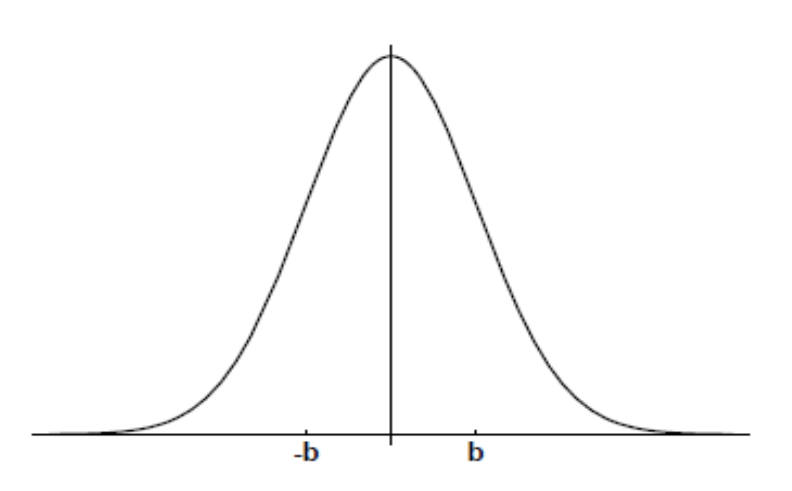
\includegraphics[width=0.3\textwidth]{images/guass.png}
                \caption{设定为高斯分布的误差}
            \end{figure}
            $$ p( \widehat{\delta }_{rot1})  = N\left( {{\widetilde{\delta }}_{{rot}1};0,{\alpha }_{1}\left| {\delta }_{{rot}1}\right|  + {\alpha }_{2}\left| {\delta }_{trans}\right| }\right) $$
            $$ p\left( {\widetilde{\mathbf{\delta }}}_{\text{trans }}\right)  = N\left( {{\widetilde{\mathbf{\delta }}}_{\text{trans }};0,{\alpha }_{3}\left| {\mathbf{\delta }}_{\text{trans }}\right|  + {\alpha }_{4}\left| {{\mathbf{\delta }}_{\text{rot1 }} + {\mathbf{\delta }}_{\text{rot2 }}}\right| }\right) $$
            $$ p\left( {\widetilde{\delta }}_{rot2}\right)  = N\left( {{\widetilde{\delta }}_{rot2};0,{\alpha }_{1}\left| {\delta }_{rot2}\right|  + {\alpha }_{2}\left| {\delta }_{trans}\right| }\right) $$
                        {\small\kaishu 
            显然,平移造成的误差和旋转造成的误差不可能对所有机器人都是一比一的,因此我们设定一些参数$\alpha_i$来作为权重;对于旋转误差例如${\widetilde{\delta }}_{{rot}1}$,其误差组成包括旋转造成的旋转误差和平移造成的旋转误差两部分;平移误差同理。
            }
        \item \textbf{求解运动模型}
        
            \begin{enumerate}
                \item \textbf{测量控制值}:将里程计数据 \( {\mathbf{u}}_{t - 1} \) 表示为 \( \mathbf{\delta } = {\left( {\delta }_{rot1},{\delta }_{trans},{\delta }_{rot2}\right) }^{T} \) ,作为测量控制值
                \item \textbf{真实控制值}:根据 \( {\mathbf{x}}_{t - 1},{\mathbf{x}}_{t} \) 计算机器人的实际运动变化量 \( \widehat{\mathbf{\delta }} = {\left( {\widehat{\delta }}_{rot1},{\widehat{\delta }}_{trans},{\widehat{\delta }}_{rot2}\right) }^{T} \) ,作为真实控制值
                \item \textbf{计算误差}:在噪声的高斯分布中随机采样\footnote{sample是一个计算机函数,调用时需传参均值和方差。均值对于误差而言就是0,我们先根据里程计的读数$\delta$和$\alpha$参数,计算出误差分布的方差$\sigma^2$;用采样函数,从一个均值为0、方差为我们刚刚计算出的$\sigma^2$的正态分布中,随机抽取一个具体的误差值$\widetilde{\delta }$。}
                $${\widetilde{\delta }}_{rot1} = {sample}\left( {{\alpha }_{1}\left| {\delta }_{rot1}\right|  + {\alpha }_{2}\left| {\delta }_{trans}\right| }\right) ,{\widetilde{\delta }}_{trans} = \cdots ,{\widetilde{\delta }}_{rot2} = ... $$
                基于采样得到的噪声和测量得到的里程计值,构建机器人实际执行
                的控制指令\footnote{其实是基于采样得到的噪声和测量得到的里程计值,构建对机器人实际发生的物理运动$\widehat{\delta }$的一次随机估计}
                $$ {\widehat{\delta }}_{rot1} = {\delta }_{rot1} - {\widetilde{\delta }}_{rot1},{\widehat{\delta }}_{trans} = {\delta }_{trans} - {\widetilde{\delta }}_{trans},{\widehat{\delta }}_{rot2} = {\delta }_{rot2} - {\widetilde{\delta }}_{rot2} $$               
                \item \textbf{估计分布}:根据真实值与测量值之间误差 \( \widetilde{\delta } = \delta  - \widehat{\delta } \) 的分布估计 \( {\mathbf{x}}_{t} \) 的分布
                
                $$ \boxed{p\left( {{\mathbf{x}}_{t} \mid  {\mathbf{x}}_{t - 1},{\mathbf{u}}_{t - 1}}\right)  = p\left( {\widetilde{\delta }}_{rot1}\right)  \cdot  p\left( {\widetilde{\delta }}_{trans}\right)  \cdot  p\left( {\widetilde{\delta }}_{rot2}\right)} $$
                \item \textbf{重复计算}:重复上述过程,所得 \( {\mathbf{x}}_{t} \) 点集合构成对 \( p\left( {{\mathbf{x}}_{t} \mid  {\mathbf{x}}_{t - 1},{\mathbf{u}}_{t - 1}}\right) \) 的描述

            \end{enumerate}
                {\small\kaishu 
                为了求解运动模型,如果正向直接求解条件概率无疑是困难的。逆向思考,如果给定$p(\mathrm{x}_t,\mathrm{x}_{t-1},\mathrm{u}_{t-1})$,能导致这种变化的随机误差也应该是唯一的。即对于一组给定的 \( \left( {{\mathbf{x}}_{t - 1},{\mathbf{u}}_{t - 1},{\mathbf{x}}_{t}}\right) \) ,存在一个唯一确定的误差值 \( \widetilde{\delta } \) 与之对应。因此,观察到特定位姿 \( {\mathbf{x}}_{t} \) 的概率,等价于发生了那个能够导致 \( {\mathbf{x}}_{t} \) 出现的唯一误差 \( \widetilde{\delta } \) 的概率。\\
                }
                \begin{figure}[H]
                \centering
                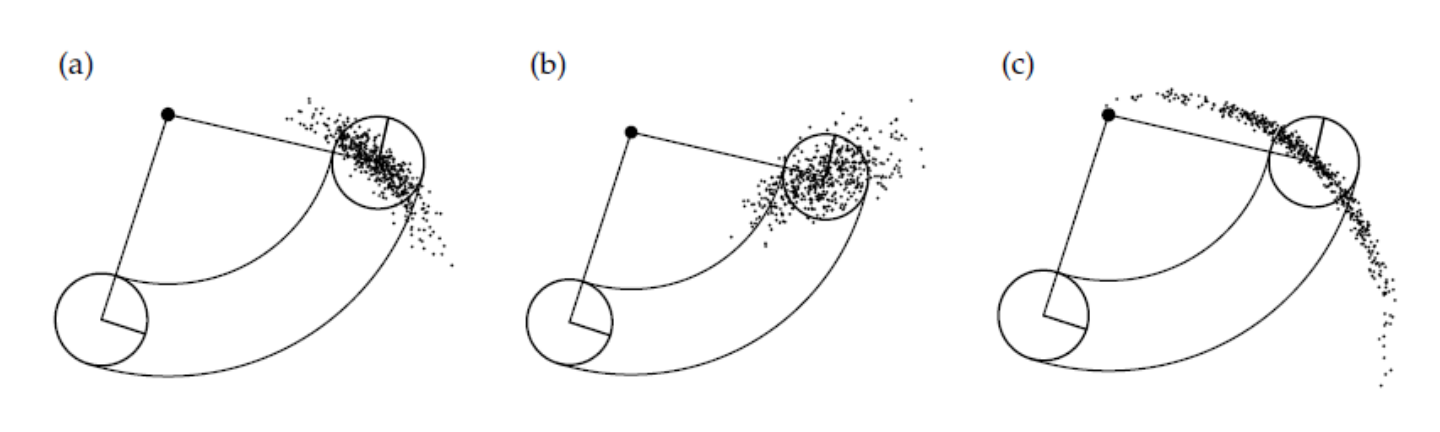
\includegraphics[width=0.6\textwidth]{images/alpha.png}
                \caption{不同$\alpha_i$参数下得到的$p(\mathrm{x}_t,\mathrm{x}_{t-1},\mathrm{u}_{t-1})$,每个子图含500个样本}
                \end{figure}
    \end{enumerate}
    \item \textbf{速度运动模型}
\end{enumerate}
\textcolor{red}{如果只考虑运动模型进行位姿估计,其不确定性(方差)会不断地无上限增大}
                    \begin{figure}[H]
                    \centering
                    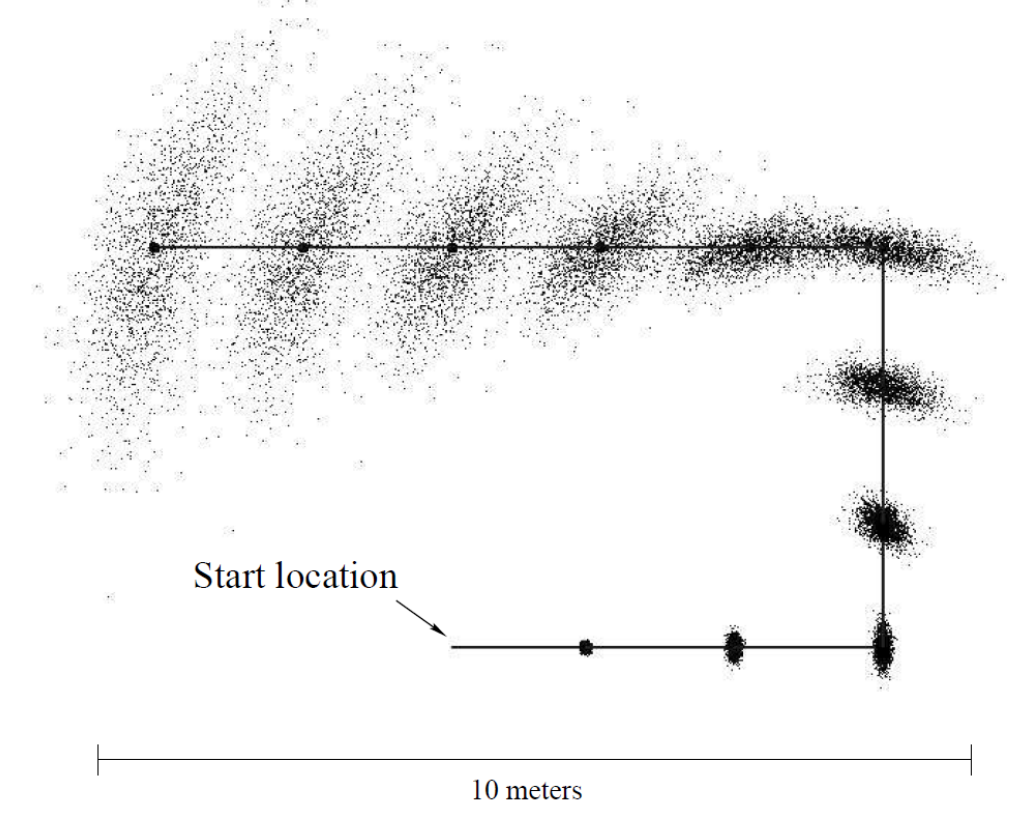
\includegraphics[width=0.4\textwidth]{images/unsure.png}
                    \caption{只用运动模型,误差不断累积}
                \end{figure}
\subsection{马尔可夫定位中的观测模型}
        \[
        p(\mathbf{x}_t \mid \mathbf{Z}^{t}, \mathbf{U}^{t-1}, \mathbf{m})
        = \eta \,\textcolor{red}{ p(\mathbf{z}_t \mid \mathbf{x}_t, \mathbf{m})}
        \int p(\mathbf{x}_t \mid \mathbf{x}_{t-1}, \mathbf{u}_{t-1}, \mathbf{m})
        \, p(\mathbf{x}_{t-1} \mid \mathbf{Z}^{t-1}, \mathbf{U}^{t-2}, \mathbf{m})
        \, d\mathbf{x}_{t-1}
        \]
            
\begin{enumerate}
    \item \textbf{特征传感器模型和观测模型}
    \item \textbf{基于物理建模的激光传感器模型}
    \item \textbf{基于Likelihood Field的激光束模}
\end{enumerate}

\end{document}